%%%%%%%%%%%%%%%%%%%%%%%%%%%%%%%%%%%%%%%%%%%%%%%%%%%%%%%%%%%%%%%%%%%%%%%%%%%%%%%%%%%%
% Styles
%
% \textit{}
% \footnotemark~
% \footnotetext{}
% \url{}
% \textbf{}
% \noindent
% \begin{itemize}[nosep]
%		\item
% \end{itemize}
% \hyperlink{page.9}{page~9~(DSPL)}
%%%%%%%%%%%%%%%%%%%%%%%%%%%%%%%%%%%%%%%%%%%%%%%%%%%%%%%%%%%%%%%%%%%%%%%%%%%%%%%%%%%%

\documentclass[runningheads,a4paper]{llncs}
\usepackage{amssymb}
\setcounter{tocdepth}{3}
\usepackage{graphicx}
\usepackage{amssymb}
\usepackage{enumitem}
\usepackage[utf8]{inputenc}
\usepackage[hidelinks]{hyperref}
\usepackage{url}
\usepackage{float}
\usepackage{amsmath}
\usepackage{graphicx}
\usepackage{wrapfig}
\usepackage{fancyhdr}
\usepackage{titling}
\usepackage{xcolor}
\usepackage{lipsum}
\newcommand{\robospecs}{%
	\newpage%
	\pagenumbering{gobble}%
	\pagestyle{fancy}%
	\fancyhf{}%
	\rhead{$|$\footnotesize\thetitle}%
	\lhead{\footnotesize\theauthor }%
	\rfoot{Robot software and hardware specification sheet}%
}


%%%%%%%%%%%%%%%%%%%%%%%%%%%%%%%%%%%%%%%%%%%%%%%%%%%%%%%%%%%%%%%%%%%%%%%%%%%%%%%%%%%%
% Title
%
% Team Description Paper submitted for qualification in the 2020 RoboCup@Home international competition to be held in Bordeaux, France.
%%%%%%%%%%%%%%%%%%%%%%%%%%%%%%%%%%%%%%%%%%%%%%%%%%%%%%%%%%%%%%%%%%%%%%%%%%%%%%%%%%%%
\title{AZ5 2020 Team Description Paper}

\author{Main author \and Co-author \and Team Members}
\institute{Complubot, \\
\texttt{http://www.complubot.com/projects/az5/}}


\begin{document}
\maketitle

%%%%%%%%%%%%%%%%%%%%%%%%%%%%%%%%%%%%%%%%%%%%%%%%%%%%%%%%%%%%%%%%%%%%%%%%%%%%%%%%%%%%
% Abstract
%
%	Max: 250 word
% Paragraphs:
% - Introduction and relevance
% - Approach
% - Contributions
% Main research line, scientific achievements, problems solved and research group focus
% Approach to the problem solution and results expected to obtain
%%%%%%%%%%%%%%%%%%%%%%%%%%%%%%%%%%%%%%%%%%%%%%%%%%%%%%%%%%%%%%%%%%%%%%%%%%%%%%%%%%%%
\begin{abstract}
We present a custom made robotics platform that aims to be low cost, ROS compatible and suited for robotics researchers.
As a prove of concept the team uses it to develop and test their algorithms.
Along the paper we will focus on the software developed for the platform as well as the software developed for this and other competitions.

The research line of the team is oriented to online object and person recognition, identification, tracking and reidentification.
To do so we use convolutional neural networks, feature extraction and feature matching, optical flow and color processing techniques.
We combine the partial results of the different algorithms with a kalman like filter to estimate the best action that the robot should perform to follow a selected target.
The target could be totally or partially occluded to the robot sight but it will keep tracking down the target even with slow rates of new images compared with the robot's control cycle rates. 

The researcher community has a great interest on these topics, specially on the robotics field.
It is our goal to contribute with a robotics platform that is capable of solving this tasks which are a solid base for other areas like person interaction or tridimensional recognition.
The platform will provide not only the hardware requirements to investigate in this fields but also our implementations to solve these problems.
\end{abstract}

%%%%%%%%%%%%%%%%%%%%%%%%%%%%%%%%%%%%%%%%%%%%%%%%%%%%%%%%%%%%%%%%%%%%%%%%%%%%%%%%%%%%
% Content
%
% Max: 8 pages
% Detailed information on the on the technical and scientific approach of the team's research.
% Current research, clearly stating all scientific contribution, and why are they important for you and the league
%%%%%%%%%%%%%%%%%%%%%%%%%%%%%%%%%%%%%%%%%%%%%%%%%%%%%%%%%%%%%%%%%%%%%%%%%%%%%%%%%%%%
\section{Introduction}
Our goal is to create an affordable and customizable platform suited for robotics researchers.
The platform is specially oriented to solve problems in the computer vision oriented towards robotics field.
The research team uses this platform to investigate in this fields so the platform keeps improving to fullfil their requirements.

This approach is quite different to the one that the software robotics community has.
We strongly believe that the hardware should adapt to the software researchers by providing them with what they need by been customizable and creating as less limitations as possible.

%%%%%%%%%%%%%%%%%%%%%%%%%%%%%%%%%%%%%%%%%%%%%%%%%%%%%%%%%%%%%%%%%%%%%%%%%%%%%%%%%%%%
% Robot description
%
% Unless your research revolves around hardware design and implementation, it is better to omit this section
% Avoid explaining ROS
% Keep it simple, more descriptive and less analytic.
% The main goal of a TDP is tell others about your latest practical achievement, what strategy was chosen and why, while at the same time trying to convince your reader that what you are doing is useful or applicable in a daily life scenario
%%%%%%%%%%%%%%%%%%%%%%%%%%%%%%%%%%%%%%%%%%%%%%%%%%%%%%%%%%%%%%%%%%%%%%%%%%%%%%%%%%%%
\subsection{Robot description}
We will leave for the annex the hardware and components details, but will address here the main ideas that had oriented the design of the platform.
Our design is oriented to be suited for robots whose main focus is image capturing.

The robot has an omnidirectional motor platform with mecanum wheels.
It is capable to reach high speeds up to 1 meter per second but also to be able to move at slower but still controlled velocities.
These features are crucial to be able to follow a person that is moving at a normal indore speed.
With this type of motor platform the robot will be able to follow its target or even to walk along it.
This type of behavior is not often achievable with other motor platform on the market so there is not currently much research of this type of human-machine interaction.
Also mecanum wheels makes our platform capable of move a total of 50kg minus the platform's weight.

Motor platforms are usually closed without offering much room for hardware modifications.
Our approach is quite different and we spect the users of our platform to have the intention of adding new hardware to it.
With this in mind our platform is powered with a fully featured computer leaving room for another one.
The battery system is capable of maintaining both computers as well as the sensors and actuators providing extra outlets for more devices.
There is room to add cameras or other sensors to the platform and place them at a desired height.

%%%%%%%%%%%%%%%%%%%%%%%%%%%%%%%%%%%%%%%%%%%%%%%%%%%%%%%%%%%%%%%%%%%%%%%%%%%%%%%%%%%%
% Achievements
%
% One paragraph to summarize the experience and achievements of your team.
% The main focus should be on describing the solution and not the team.
%%%%%%%%%%%%%%%%%%%%%%%%%%%%%%%%%%%%%%%%%%%%%%%%%%%%%%%%%%%%%%%%%%%%%%%%%%%%%%%%%%%%
\subsection{Team achievements}



%%%%%%%%%%%%%%%%%%%%%%%%%%%%%%%%%%%%%%%%%%%%%%%%%%%%%%%%%%%%%%%%%%%%%%%%%%%%%%%%%%%%
% Content
%
% Innovative technology and scientific contribution
% Focus of research/research interests
% Re-usability of the system for other research groups
% Applicability of the robot in the real world
% When the robot depicted in the TDP or Team Video is different from the league's standard one, the TDP must clearly state how the addressed approach and described software will be adapted to the standard platform robot.
% Everything must be in perfect standard scientific English
%%%%%%%%%%%%%%%%%%%%%%%%%%%%%%%%%%%%%%%%%%%%%%%%%%%%%%%%%%%%%%%%%%%%%%%%%%%%%%%%%%%%
\section{Main research}
In this section we will target the software created by the research team for the platform and in the field of robot computer vision.


%%%%%%%%%%%%%%%%%%%%%%%%%%%%%%%%%%%%%%%%%%%%%%%%%%%%%%%%%%%%%%%%%%%%%%%%%%%%%%%%%%%%
% Implemented algorithms transversal to the latest research that are also used
%%%%%%%%%%%%%%%%%%%%%%%%%%%%%%%%%%%%%%%%%%%%%%%%%%%%%%%%%%%%%%%%%%%%%%%%%%%%%%%%%%%%
\section{Other relevant contributions}



\section{Experiments and results}



\section{Conclusions and future work}



%%%%%%%%%%%%%%%%%%%%%%%%%%%%%%%%%%%%%%%%%%%%%%%%%%%%%%%%%%%%%%%%%%%%%%%%%%%%%%%%%%%%
% Bibliography
%%%%%%%%%%%%%%%%%%%%%%%%%%%%%%%%%%%%%%%%%%%%%%%%%%%%%%%%%%%%%%%%%%%%%%%%%%%%%%%%%%%%
\newpage
\bibliographystyle{unsrt}
\bibliography{bibliography}

\newpage
\robospecs

%%%%%%%%%%%%%%%%%%%%%%%%%%%%%%%%%%%%%%%%%%%%%%%%%%%%%%%%%%%%%%%%%%%%%%%%%%%%%%%%%%%%
% OPL Annex
%
% Recommended 1 page
% The TDP's Robot Description Annex is an appendix of arbitrary length that must be attached at the end of the TDP and summarize the robot's software and hardware technical specifications.
% In this section briefly describe the software and hardware of the robot
%
% Purpose
% It allows the league to track changes in hardware and software trends over time.
% It helps experienced teams to find alternatives to their solutions when looking to improve or conducting benchmarking.
% It serves as a quick reference guide for new teams while preparing their robots.
%%%%%%%%%%%%%%%%%%%%%%%%%%%%%%%%%%%%%%%%%%%%%%%%%%%%%%%%%%%%%%%%%%%%%%%%%%%%%%%%%%%%

%%%%%%%%%%%%%%%%%%%%%%%%%%%%%%%%%%%%%%%%%%%%%%%%%%%%%%%%%%%%%%%%%%%%%%%%%%%%%%%%%%%%
% Parts of the robot
% Devices: bateries, motors, arms, cameras, lidar...
%%%%%%%%%%%%%%%%%%%%%%%%%%%%%%%%%%%%%%%%%%%%%%%%%%%%%%%%%%%%%%%%%%%%%%%%%%%%%%%%%%%%
\section*{Robot's Hardware Description}
\label{sec:annex-OPL}


%%%%%%%%%%%%%%%%%%%%%%%%%%%%%%%%%%%%%%%%%%%%%%%%%%%%%%%%%%%%%%%%%%%%%%%%%%%%%%%%%%%%
% Photo of the robot
%%%%%%%%%%%%%%%%%%%%%%%%%%%%%%%%%%%%%%%%%%%%%%%%%%%%%%%%%%%%%%%%%%%%%%%%%%%%%%%%%%%%
\setlength\intextsep{0pt}
\begin{wrapfigure}[10]{r}{0.3\textwidth}
	\centering
	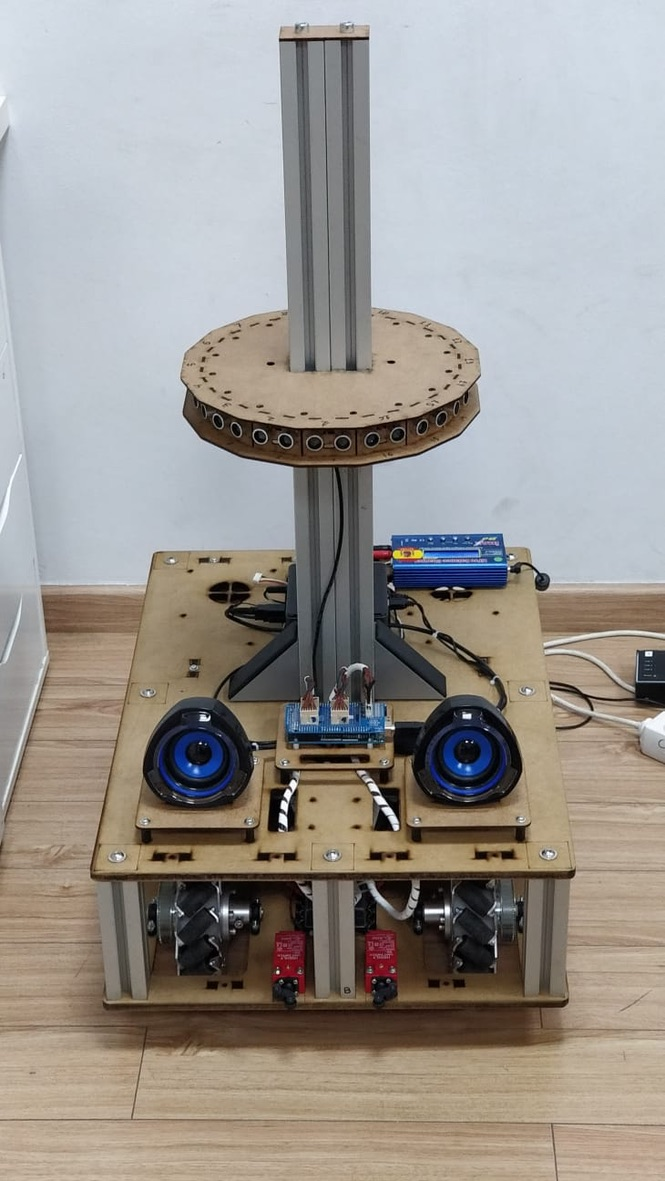
\includegraphics[width=0.4\textwidth]{images/AZ5.jpeg}
	\caption{AZ5}
	\label{fig:wall-e}
\end{wrapfigure}

%%%%%%%%%%%%%%%%%%%%%%%%%%%%%%%%%%%%%%%%%%%%%%%%%%%%%%%%%%%%%%%%%%%%%%%%%%%%%%%%%%%%
% Robot SW
% Platform:Operating System
% Navigation
% Recognition
% Speech recognition
% Speech generation
% Arms control...
%%%%%%%%%%%%%%%%%%%%%%%%%%%%%%%%%%%%%%%%%%%%%%%%%%%%%%%%%%%%%%%%%%%%%%%%%%%%%%%%%%%%
\section*{Robot's Software Description}



%%%%%%%%%%%%%%%%%%%%%%%%%%%%%%%%%%%%%%%%%%%%%%%%%%%%%%%%%%%%%%%%%%%%%%%%%%%%%%%%%%%%
% External devices
% 
% Cloud computing
% External computing or actuators
%%%%%%%%%%%%%%%%%%%%%%%%%%%%%%%%%%%%%%%%%%%%%%%%%%%%%%%%%%%%%%%%%%%%%%%%%%%%%%%%%%%%
\section*{External Devices}



%%%%%%%%%%%%%%%%%%%%%%%%%%%%%%%%%%%%%%%%%%%%%%%%%%%%%%%%%%%%%%%%%%%%%%%%%%%%%%%%%%%%
% SAS
%
% Geolocalization
% Language processing
%%%%%%%%%%%%%%%%%%%%%%%%%%%%%%%%%%%%%%%%%%%%%%%%%%%%%%%%%%%%%%%%%%%%%%%%%%%%%%%%%%%%
\section*{Cloud Services}

\nocite{*}
\end{document}
